\documentclass[border=12pt]{standalone}
\usepackage{tikz}
\usetikzlibrary{shapes.geometric, arrows.meta, positioning, calc, fit, backgrounds}
\usepackage{fontspec}
\usepackage{amsmath,amssymb}
\setmainfont{DejaVu Sans}

\begin{document}
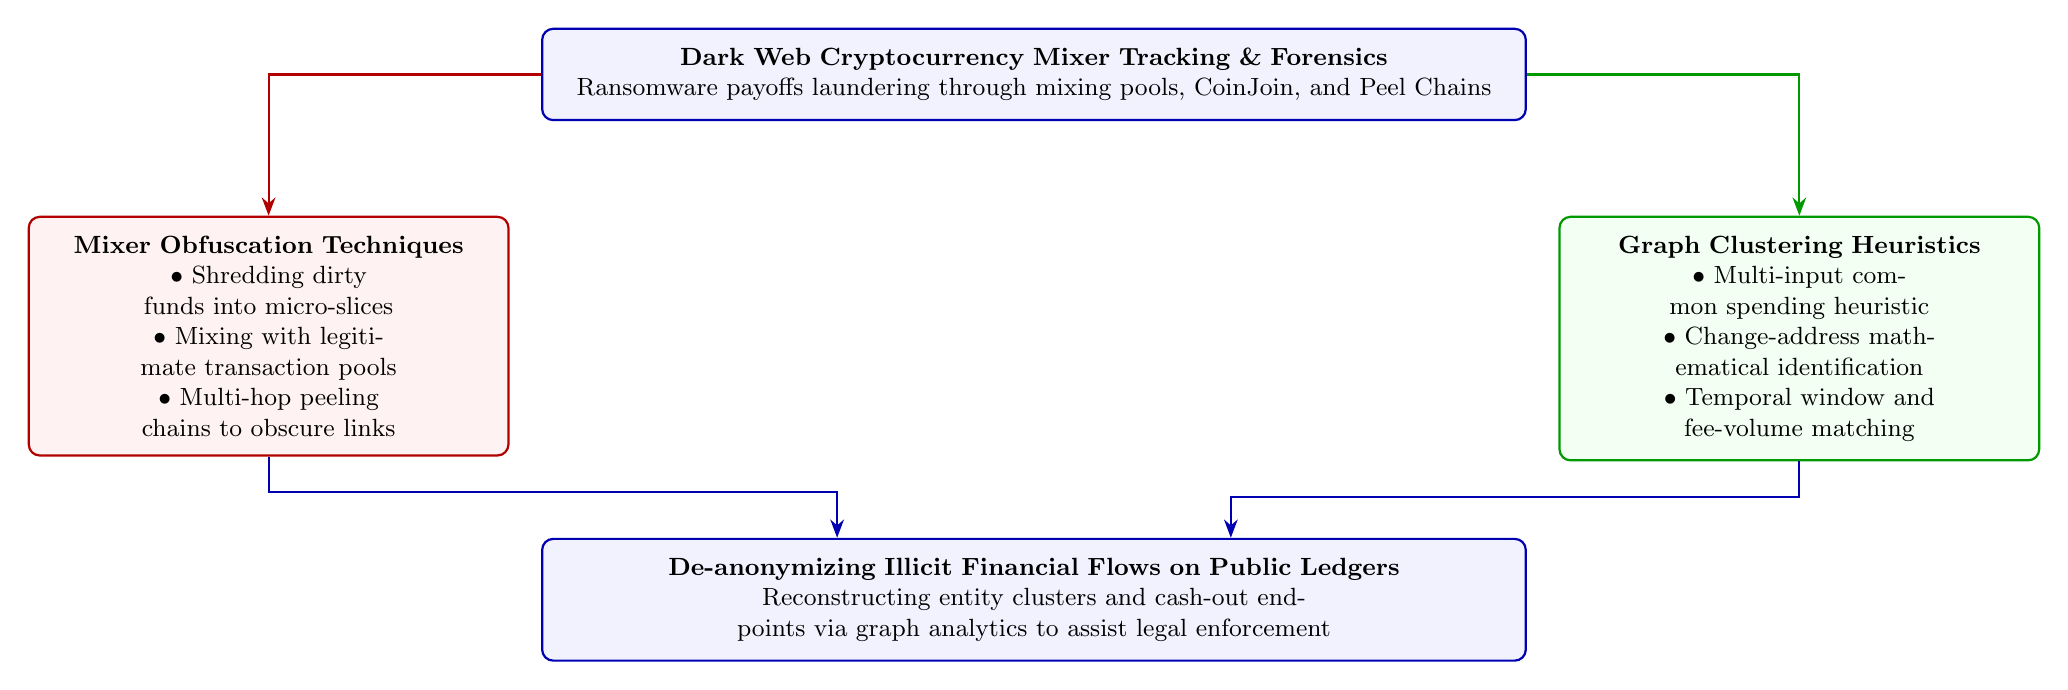
\begin{tikzpicture}[
    font=\small,
    >=Stealth,
    node distance=1.2cm,
    block/.style={rectangle, draw=blue!70!black, fill=blue!5, rounded corners=4pt, thick, align=center, inner sep=7pt},
    alertblock/.style={rectangle, draw=red!70!black, fill=red!5, rounded corners=4pt, thick, align=center, inner sep=7pt},
    greenblock/.style={rectangle, draw=green!60!black, fill=green!5, rounded corners=4pt, thick, align=center, inner sep=7pt},
    amberblock/.style={rectangle, draw=orange!80!black, fill=orange!5, rounded corners=4pt, thick, align=center, inner sep=7pt}
]

\node[block, text width=12cm] (top) {\textbf{Dark Web Cryptocurrency Mixer Tracking \& Forensics}\\Ransomware payoffs laundering through mixing pools, CoinJoin, and Peel Chains};

\node[alertblock, below left=1.2cm and 0.4cm of top, text width=5.6cm] (mixer) {\textbf{Mixer Obfuscation Techniques}\\$\bullet$ Shredding dirty funds into micro-slices\\$\bullet$ Mixing with legitimate transaction pools\\$\bullet$ Multi-hop peeling chains to obscure links};

\node[greenblock, below right=1.2cm and 0.4cm of top, text width=5.6cm] (graph) {\textbf{Graph Clustering Heuristics}\\$\bullet$ Multi-input common spending heuristic\\$\bullet$ Change-address mathematical identification\\$\bullet$ Temporal window and fee-volume matching};

\node[block, below=1.0cm of $(mixer.south)!0.5!(graph.south)$, text width=12cm] (bottom) {\textbf{De-anonymizing Illicit Financial Flows on Public Ledgers}\\Reconstructing entity clusters and cash-out endpoints via graph analytics to assist legal enforcement};

\draw[->, thick, red!70!black] (top) -| (mixer);
\draw[->, thick, green!60!black] (top) -| (graph);
\draw[->, thick, blue!70!black] (mixer.south) -- ++(0,-0.45) -| ([xshift=-2.5cm]bottom.north);
\draw[->, thick, blue!70!black] (graph.south) -- ++(0,-0.45) -| ([xshift=2.5cm]bottom.north);

\end{tikzpicture}
\end{document}
